%Author Alex Clemmer
%CS 3810 Computer Organization
%Assignment 6:
\documentclass[a4paper]{article}
\usepackage[pdftex]{graphicx}
\usepackage{fancyvrb}
\usepackage{multirow}
\usepackage{amssymb}
\usepackage{amsmath}
\usepackage{fullpage}
\addtolength{\oddsidemargin}{-.05in}
	\addtolength{\evensidemargin}{-.05in}
	\addtolength{\textwidth}{.25in}

	\addtolength{\textheight}{.25in}
\begin{document}

\section*{Assignment 6 }
Alex Clemmer\\
Student number: u0458675

\section{Problem 1:}

\begin{center}
\begin{tabular}{|c|c|c|c|c|c|c|c|c|}
\hline
& $\textit{RegDst}$ & $\textit{Branch}$ & $\textit{MemRead}$ & $\textit{MemtoReg}$ & $\textit{ALUOp}$ & $\textit{MemWrite}$ & $\textit{ALUSrc}$ & $\textit{RegWrite}$  \\
\hline
\hline
$\texttt{ori}$ & $\texttt{0}$ & $\texttt{0}$ & $\texttt{0}$ & $\texttt{0}$ & $\texttt{or}$ & $\texttt{0}$ & $\texttt{1}$ & $\texttt{1}$ \\
\hline
$\texttt{add}$ & $\texttt{1}$ & $\texttt{0}$ & $\texttt{0}$ & $\texttt{0}$ & $\texttt{add}$ & $\texttt{0}$ & $\texttt{0}$ & $\texttt{1}$ \\
\hline
$\texttt{lw}$ & $\texttt{0}$ & $\texttt{0}$ & $\texttt{1}$ & $\texttt{1}$ & $\texttt{add}$ & $\texttt{0}$ & $\texttt{1}$ & $\texttt{1}$ \\
\hline
$\texttt{sw}$ & $\texttt{x}$ & $\texttt{0}$ & $\texttt{0}$ & $\texttt{x}$ & $\texttt{add}$ & $\texttt{1}$ & $\texttt{1}$ & $\texttt{0}$ \\
\hline
$\texttt{beq}$  & $\texttt{x}$ & $\texttt{1}$ & $\texttt{0}$ & $\texttt{x}$ & $\texttt{sub}$ & $\texttt{0}$ & $\texttt{0}$ & $\texttt{0}$ \\
\hline
\end{tabular}
\end{center}

\section{Problem 2:}

Here we add several things. First, we branch off immediately after fetching the instruction, and shift the lower 26 bits of the instruction left 2 bits. We then concatenate the upper 4 bits of the PC+4 and place those as the most significant bits in the instruction.

Why? In MIPS, $\texttt{jal}$ is by offset, so we need to put the top of the PC onto the jump location. The low order bits are always a $\texttt{00}$ for a jump.

A new mux should then mux this result with whatever the output of the branch/increment mux is, and the result should be that we end up routing this "new" address to the PC. To manage this new mux, we add a control line called "jump".

Also worth noting is that immediately to the left of the register file is a new mux that muxes the result of the mux that was already there with the value 31. This is provided because $\texttt{jal}$ can't provide fields that specify the $\texttt{\$ra}$. When this is selected, we are telling the register file that we want to write to register 31.

From there, we will proceed through the control path normally until we are ready to write back to the register. You will notice at the bottom is another mux, which muxes the output of the mux that determines whether we write the result of the ALU or memory to an address. This mux determines whether we will write that output, or the current PC+4.

For the record, I chose to implement $\texttt{jump}$ and $\texttt{jal}$ separately, but we would also need to implement $\texttt{jr}$ to use $\texttt{\$ra}$ to jump back. Oops!

One more thing: A $\texttt{jal}$ call would look like this.

\begin{center}
\begin{tabular}{|c|c|c|c|c|c|c|c|c|c|}
\hline
$\textit{RegDst}$ & $\textit{Branch}$ & $\textit{MemRead}$ & $\textit{MemtoReg}$ & $\textit{ALUOp}$ & $\textit{MemWrite}$ & $\textit{ALUSrc}$ & $\textit{RegWrite}$ & $\textit{jump}$ & $\textit{jal}$ \\
\hline
$\texttt{x}$ & $\texttt{x}$ & $\texttt{x}$ & $\texttt{x}$ & $\texttt{x}$ & $\texttt{0}$ & $\texttt{x}$ & $\texttt{1}$ & $\texttt{1}$ & $\texttt{1}$ \\
\hline
\end{tabular}
\end{center}

It's helpful to note that, strictly speaking, we require none of those fields to be filled in, but they should be filled in and NOT accessed unless necessary. In other words, this chart could have looked a lot like the one above, but I felt like the criteria was vague enough that I couldn't justify excluding some and not excluding others.

(picture on next page)

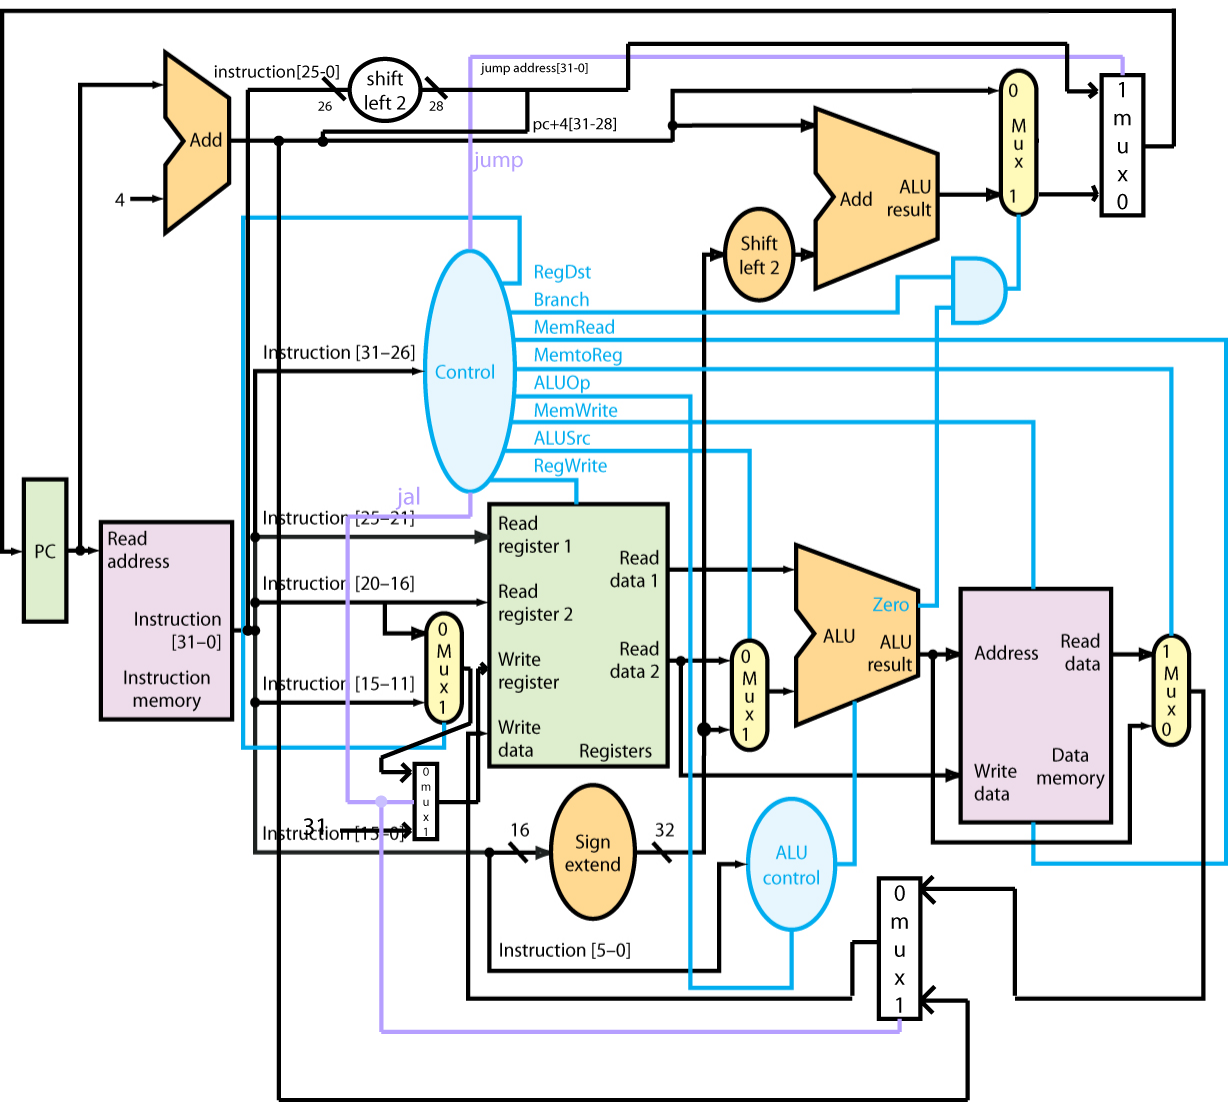
\includegraphics[width=150mm]{cpu.png}

\section{Problem 3:}

Both of these are pretty straightforward:

\paragraph{(a) \\} 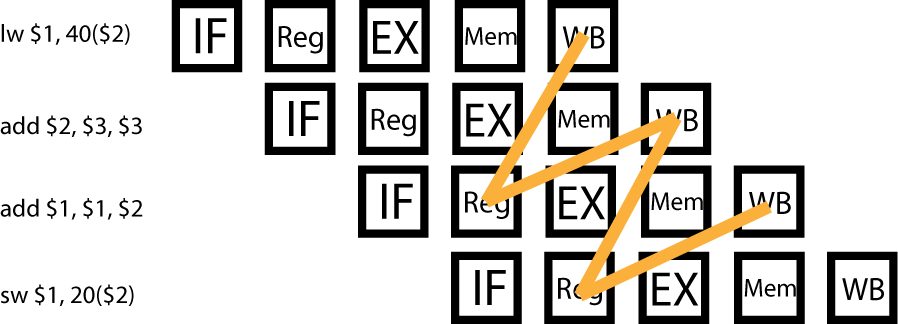
\includegraphics[width=100mm]{p3_a.png}

\paragraph{(b) \\} 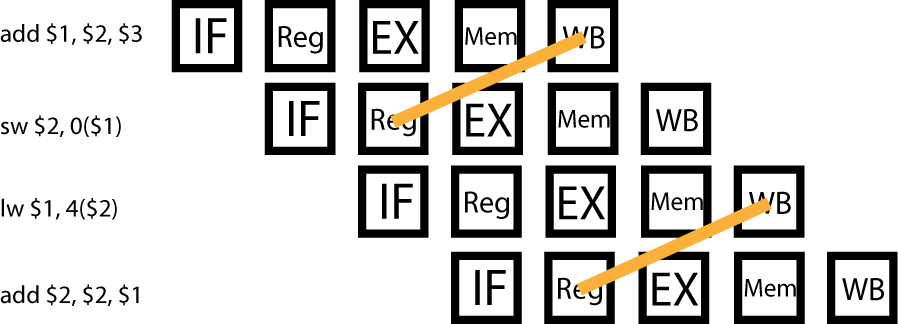
\includegraphics[width=100mm]{p3_b.png}

\section{Problem 4:}

These, once again, are pretty straightforward:

\paragraph{(a) \\} 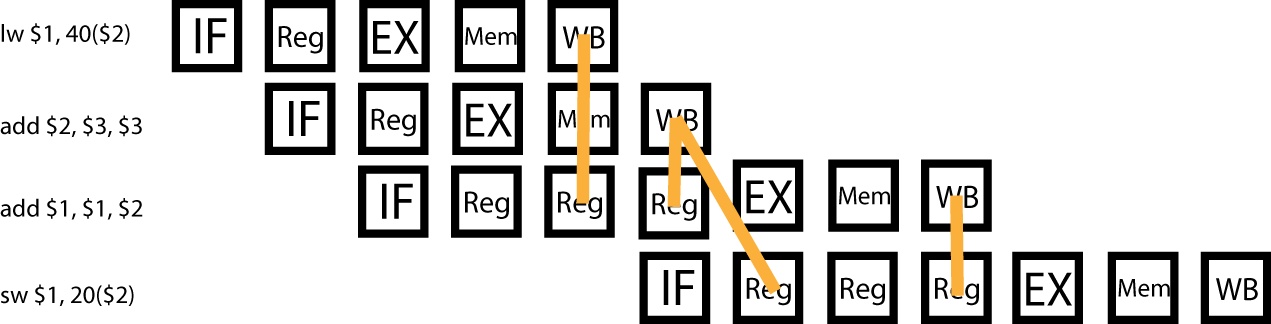
\includegraphics[width=150mm]{p4_a.png}

\paragraph{(b) \\} 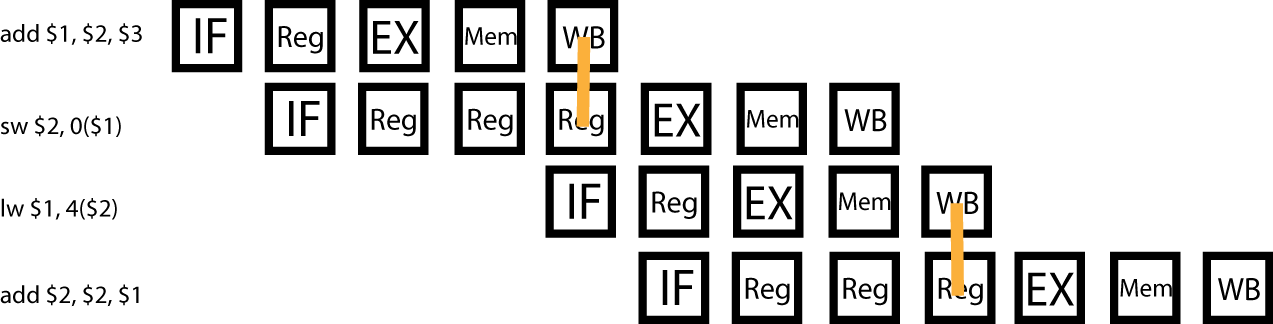
\includegraphics[width=150mm]{p4_b.png}

\section{Problem 5 and 6:}

NOTE that I've combined them into one diagram for simplicity.

\paragraph{(a) \\} 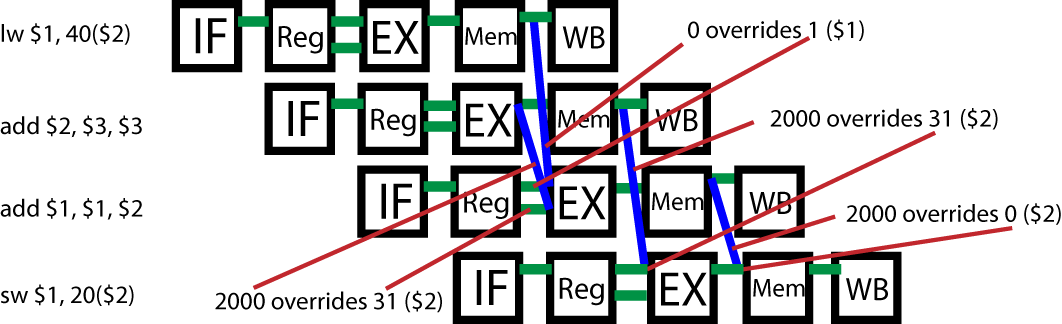
\includegraphics[width=150mm]{p5_a.png}

\paragraph{(b) \\} 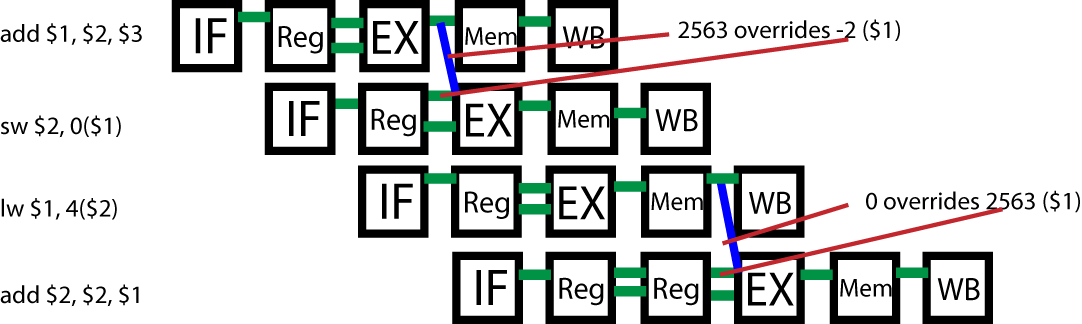
\includegraphics[width=150mm]{p5_b.png}


\end{document}